\section{Methods}
\label{sec:methods}

% Kept in step with docs/methods.md and the code. Change both in the same pull request.

\subsection{Study design}

Each experiment arm redocks every complex of the benchmark set under one preparation
protocol and scores the top-ranked pose. Arms differ from a baseline in exactly one
preparation choice, so a difference in outcome can be attributed to that choice. All arms
are run on the same complexes and compared with paired statistics
(Figure~\ref{fig:design}).

\begin{figure}[t]
  \centering
  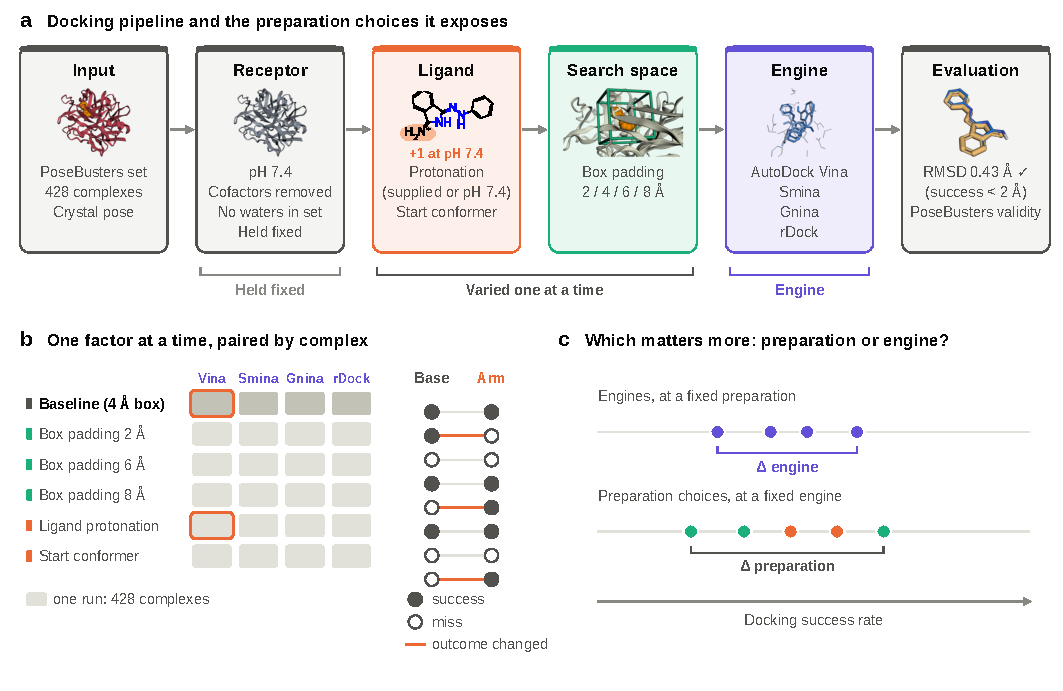
\includegraphics[width=\textwidth]{concept_v4.pdf}
  \caption{Study design. \textbf{(a)}~Redocking pipeline, shown for complex 5SAK\_ZRY: each
    complex passes through receptor preparation (held fixed: pH 7.4, cofactors removed; the
    dataset contains no waters), ligand preparation (here protonation at pH 7.4 adds a
    positive charge, highlighted) and search-space definition (the box around the crystal
    ligand), then docking with each of four engines (the four top-ranked Vina poses are
    shown). The top-ranked pose is scored by heavy-atom RMSD to the crystal ligand (success
    below \SI{2}{\angstrom}; \SI{0.43}{\angstrom} here) and by the PoseBusters checks.
    \textbf{(b)}~Each of the five arms changes one choice from the baseline
    (\SI{4}{\angstrom} box padding, supplied ligand) and is run with every engine; an arm
    is compared with the baseline of the same engine complex by complex (right: filled
    circles mark successes, orange lines complexes whose outcome changed). The outcomes
    shown are illustrative. \textbf{(c)}~The question addressed: is the spread in success
    across preparation choices comparable to the spread across engines? Positions in (c)
    are schematic, not results.}
  \label{fig:design}
\end{figure}

\subsection{Dataset}

We use the PoseBusters Benchmark set \citep{buttenschoen2024posebusters} in the version
released on Zenodo with the study's data \citep{posebusters2023data}: 428 protein--ligand
complexes. The archive is verified against its MD5 checksum. During peer review of the
PoseBusters study its authors found that some of these structures contain crystal contacts:
the ligand lies close to a symmetry-related copy of the protein (a neighbouring molecule in
the crystal lattice that is absent from the deposited protein file and so invisible to a
docking engine), which can hold it in a pose that docking against one copy cannot be
expected to reproduce. The journal version therefore reports results on the subset of 308
complexes in which no ligand atom lies within \SI{5}{\angstrom} of any symmetry mate
(\citealp{buttenschoen2024posebusters}, ESI Table S1), whose identifiers are linked from the
same Zenodo record. All 308 are among the 428. Our primary analysis uses
all 428 complexes; every comparison is repeated on the 308-complex subset as a robustness
check. For each complex the set provides the protein without
the ligand of interest, without solvent and with cofactors retained; the crystal ligand,
which defines the binding site and serves as the RMSD reference; and a start conformer of
the ligand generated by the dataset authors with RDKit, independent of the crystal pose.
Because the protein files contain no waters, retained waters cannot be studied with the set
as distributed.

\subsection{Receptor preparation}

Receptors are prepared with PDBFixer and OpenMM \citep{eastman2024openmm}. Nonstandard
residues are mutated to their standard parents and all heterogens (cofactors, ions,
crystallisation additives) are removed; missing loops are not modelled. Hydrogens present in
the input are deleted so that protonation follows the protocol alone, and residues not
bonded to any other residue are removed, since no Amber template covers a free amino acid.
Missing heavy atoms are rebuilt and hydrogens are added at the protocol's pH (baseline 7.4).
The added atoms are then relaxed by energy minimisation with OpenMM's Amber14 force field
(ff14SB for the protein \citep{maier2015ff14sb}; non-periodic, \SI{1}{\nano\metre} cutoff, at most 500 iterations) while every atom present
in the crystal structure is held fixed, so experimental coordinates are unchanged.
Without this step, initial atom placements produced spurious bonds under distance-based bond
perception for about half of the set.

All minimisations run on OpenMM's single-threaded Reference platform with a seeded random
generator. New hydrogens are otherwise placed at random positions and multithreaded force
summation is order-dependent, which together made prepared receptors differ between runs by
up to \SI{2.6}{\angstrom}; with these measures, preparation is reproducible to the byte.

For Vina, the prepared receptor is converted to rigid-receptor PDBQT with Meeko
\citep{meeko}, which matches every residue to a chemical template. A residue that fails
matching is dropped only if it lies more than \SI{8}{\angstrom} outside the search box,
Vina's interaction cutoff; otherwise the complex is recorded as a preparation failure. The
other engines read the prepared receptor directly (Smina and Gnina) or after conversion to
Mol2 with Open Babel 3.2.1 \citep{oboyle2011openbabel} (rDock), so this step is specific to
Vina.

\subsection{Ligand preparation}

Ligands are docked from the supplied start conformer. Two options are varied.
\emph{Protonation}: the supplied state is kept, or the dominant state at the protocol's pH is
assigned with Dimorphite-DL \citep{ropp2019dimorphite}, transferring charges, hydrogen counts
and bond orders onto the start conformer while its heavy atoms stay fixed. At pH 7.4 this
changes the net formal charge of 271 of the 428 ligands. \emph{Start conformer}: the supplied
conformer, or a new one generated with RDKit \citep{rdkit} (ETKDGv3 \citep{wang2020etkdgv3},
fixed seed, then MMFF94 minimisation \citep{halgren1996mmff94}). Protonation is applied before conformer generation; both options succeed for
all 428 ligands. The supplied conformer was itself generated with ETKDGv3 and minimised with
UFF \citep{rappe1992uff} by the dataset authors (\citealp{buttenschoen2024posebusters}, ESI section S1), so the
start-conformer arm draws a new conformer from a similar generator rather than replacing an
experimental geometry.

\subsection{Search space and docking}

The search box is axis-aligned and centred on the extent of the crystal ligand's heavy
atoms, padded on each side by the protocol's padding (baseline \SI{4}{\angstrom}). Every
arm is docked with four engines, each given the same prepared receptor, ligand and box and
asked for up to nine poses with a fixed seed (42):
\begin{itemize}
  \item \emph{AutoDock Vina} 1.2.7 \citep{trott2010vina,eberhardt2021vina}, through its
    Python bindings, with the Vina scoring function and exhaustiveness 8. Poses are
    converted back to RDKit molecules through Meeko, which restores bond orders.
  \item \emph{Smina} (build of 15 October 2019) \citep{koes2013smina}, a fork of Vina whose
    default scoring function reproduces Vina's, run from the command line with
    exhaustiveness 8.
  \item \emph{Gnina} 1.3.3 \citep{mcnutt2021gnina}, which searches with the Smina machinery and re-ranks the final
    poses with its default convolutional neural network ensemble (\texttt{--cnn\_scoring
    rescore}); exhaustiveness 8, on GPUs.
  \item \emph{rDock} 24.03 \citep{ruizcarmona2014rdock}, with 50 independent runs per ligand
    and the standard docking protocol shipped with rDock (\texttt{dock.prm}). rDock defines its search space as a cavity rather
    than a box, so the cavity is mapped as the free space inside the same box the other
    engines use: rDock's reference-ligand mapper is given a reference made of points at the
    centres of a regular grid filling the box (at most 999 points, at least
    \SI{1.5}{\angstrom} apart), each with a radius of half a grid-cell diagonal, so that the
    cavity covers the box and extends beyond its faces by at most a third of a cell. Poses
    are ranked by the rDock total score. rDock writes poses without formal charges and
    without all input hydrogens, so each pose's heavy atoms are matched to the input ligand
    by element and connectivity, the input ligand takes the pose's coordinates, and
    hydrogens are added back in place. Two earlier cavity definitions, a sphere enclosing
    the box and a cavity mapped around the crystal ligand, were replaced because their
    search spaces did not match the box (Supplementary Information).
\end{itemize}
All returned poses are saved with their rank, score and RMSD. Smina, Gnina and rDock run as
external programs limited to one hour per complex; a run that exceeds the limit counts as a
failure (three rDock runs, in the two largest boxes). Five rDock runs (one complex in
one arm each) that were stopped by the server's memory limit were docked again with more
memory, so every complex has a result in every arm.

\subsection{Evaluation}

Only the top-ranked pose determines success. RMSD is the symmetry-corrected heavy-atom
RMSD to the crystal ligand, computed without superposition because docked poses share the
receptor frame; atoms are matched on the heavy-atom graph ignoring formal charges, so a pose
docked in a different protonation state still matches. A pose is a \emph{top-1 success} if
its RMSD is below \SI{2}{\angstrom}, and a \emph{\pbvalid{} success} if it also passes every
PoseBusters \citep{buttenschoen2024posebusters} redocking check other than its own RMSD
check. Contacts are checked against the original protein file, with cofactors, as in the
PoseBusters protocol. A complex whose preparation or docking fails counts as a failure.

To explain differences between arms, each top pose is assigned one failure class: valid
success; correct but not \pbvalid{}; scoring failure (a pose below \SI{2}{\angstrom} exists
but is not ranked first); wrong site (the top pose's centroid lies more than
\SI{4}{\angstrom} from the crystal ligand's, a heuristic threshold); or wrong binding mode.
Classes are assigned in that order: a failed complex first, then a top pose below
\SI{2}{\angstrom} (valid or not), then a scoring failure, and only then wrong site or wrong
mode by the centroid distance, so the classes do not overlap.

\subsection{Statistics}

Success rates are reported with 95\% Wilson score intervals \citep{wilson1927}. An arm is
compared with the baseline on the complexes both share using an exact McNemar test
\citep{mcnemar1947}, a two-sided binomial test on the complexes that succeed in exactly one
of the two. P-values across the five arms tested against one baseline are adjusted with
Holm's method \citep{holm1979}, separately for each engine and each success metric. These
five arms are the study's primary comparisons; the follow-up arms described below are
analysed separately, each set with its own correction, and do not enter this family.

Effects are interpreted against the run-to-run variation of the baseline. The Vina baseline
was repeated with three further docking seeds (1, 2 and 3; preparation is identical, so only
the search differs). From the four replicates we report the spread of the success rate and
the number of complexes whose outcome changes between pairs of seeds, and an arm's count of
changed complexes is compared with that seed-to-seed count. This is a descriptive yardstick
rather than a test: every arm is itself docked with one seed, so its changes include some
stochastic ones, and four replicates cannot reveal every complex with a small chance of
flipping. Engines are compared with each other both on all 428 complexes, counting preparation
failures as failures, and on the complexes every engine docked.

To see which complexes a preparation choice affects, the complexes whose top-1 outcome
differs between an arm and its baseline (\emph{flipped}) are compared with the rest on
properties of the supplied ligand and its complex: heavy atoms, rotatable bonds,
absolute formal charge, whether protonation at pH 7.4 changes the net charge, and whether
the protein file contains a cofactor (any heterogen other than solvent, simple ions and
common crystallisation additives). For Vina, whose baseline was repeated with several
seeds, seed sensitivity (an outcome that differs between replicates) is also included.
Continuous properties are compared with the two-sided Mann--Whitney $U$ test, with the
rank-biserial correlation as effect size; binary ones with Fisher's exact test and the
odds ratio. P-values are Holm-adjusted over the properties tested for each engine and
arm. These comparisons are exploratory.

Agreement between poses is measured with the same symmetry-corrected heavy-atom RMSD, without
superposition, between the top-1 poses of two runs; two poses agree when it is below
\SI{2}{\angstrom}. For each engine, the baseline pose's agreement with the five primary arms
(0--5), with the baseline poses of the other three engines (0--3) and, for Vina, with its three
seed replicates (0--3) is compared with the docking score, and for Gnina its CNN pose score, as a
predictor of baseline top-1 success. Each signal is summarised by the area under the ROC curve,
with 95\% intervals and paired differences from 2,000 bootstrap resamples of complexes. The
consensus pose is the top-1 pose, among the baseline and the five arms, within \SI{2}{\angstrom}
of the most others, ties going to the baseline; it is compared with the baseline pose by the
exact McNemar test, with Holm's correction over the four engines for each success metric. This
analysis was conceived after the runs were complete, so it is exploratory, and its thresholds
were not tuned. It is regenerated with \texttt{python -m dockprepbench.analysis.agreement}.

All other tables are regenerated from the per-complex results with \texttt{dockprepbench report}.

\subsection{Experiment arms}

\begin{table}[h]
  \centering
  \caption{Experiment arms. Each changes one choice from the baseline.}
  \label{tab:arms}
  \begin{tabular}{ll}
    \toprule
    Arm & Change from baseline \\
    \midrule
    Baseline & pH 7.4, \SI{4}{\angstrom} padding, supplied ligand state and conformer \\
    Box padding & \SIlist{2;6;8}{\angstrom} \\
    Ligand protonation & Dominant state at pH 7.4 (Dimorphite-DL) \\
    Start conformer & Regenerated with RDKit \\
    \bottomrule
  \end{tabular}
\end{table}

\paragraph{Follow-up arms (Vina only).} Two further sets of runs test assumptions of the
one-factor design. First, ligand protonation at pH 7.4 is repeated at 2, 6 and
\SI{8}{\angstrom} padding. At each padding it is compared with the same padding without
protonation (exact McNemar, Holm-adjusted over the four paddings, the \SI{4}{\angstrom}
comparison being the primary protonation arm). Whether its effect depends on the padding is
tested complex by complex: for each complex the effect at a padding (+1, 0 or $-1$) minus its
effect at \SI{4}{\angstrom} is computed, and the non-zero differences are tested with a
two-sided sign test, Holm-adjusted over the three paddings. Second, the box is sized to the
ligand following \citet{feinstein2015boxsize}: a cube whose edge is 2.857 times the radius of
gyration of the docked conformer's heavy atoms (unweighted), centred on the centroid of the
crystal ligand's heavy atoms rather than on the centre of its extent. The combined protocol
and this box are compared with the baseline and with the \SI{2}{\angstrom} box by exact
McNemar tests without further adjustment; these comparisons are exploratory.

\subsection{Reproducibility}

Each run records its configuration, engine settings, software version and timestamps
alongside its results. Dependencies are pinned in a lock file (Python 3.12, RDKit 2026.09,
Meeko 0.8, Vina 1.2.7, OpenMM 8.6, PDBFixer 1.12, PoseBusters 0.6.5, Dimorphite-DL 2.1).
Receptor preparation, ligand preparation and docking with Vina, Smina and rDock are
deterministic for given inputs and versions; Gnina's neural-network scores, computed on
GPUs, may differ in the last digits between hardware. External engines are installed by \texttt{scripts/setup.sh} in the repository.
Runs were carried out on a shared Linux server (Ubuntu 22.04) with one complex per worker
process; Gnina used NVIDIA GPUs. Each run writes a per-complex checkpoint, so an interrupted
run resumes without redocking finished complexes.
